% This file was created with tikzplotlib v0.9.12.
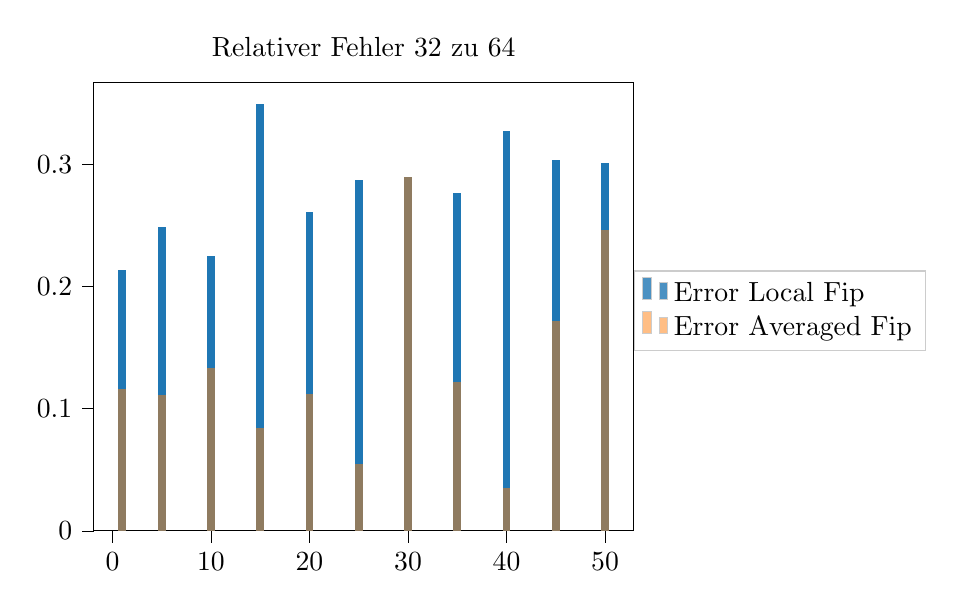
\begin{tikzpicture}

\definecolor{color0}{rgb}{0.12156862745098,0.466666666666667,0.705882352941177}
\definecolor{color1}{rgb}{1,0.498039215686275,0.0549019607843137}

\begin{axis}[
legend cell align={left},
legend style={
  fill opacity=0.8,
  draw opacity=1,
  text opacity=1,
  at={(1,0.4)},
  anchor=south west,
  draw=white!80!black
},
tick align=outside,
tick pos=left,
title={Relativer Fehler 32 zu 64},
x grid style={white!69.0196078431373!black},
xmin=-1.89, xmax=52.89,
xtick style={color=black},
y grid style={white!69.0196078431373!black},
ymin=0, ymax=0.366887181588989,
ytick style={color=black}
]
\draw[draw=none,fill=color0] (axis cs:0.6,0) rectangle (axis cs:1.4,0.213565747920035);
\addlegendimage{ybar,ybar legend,draw=none,fill=color0}
\addlegendentry{Error Local Fip}

\draw[draw=none,fill=color0] (axis cs:4.6,0) rectangle (axis cs:5.4,0.248305663546967);
\draw[draw=none,fill=color0] (axis cs:9.6,0) rectangle (axis cs:10.4,0.225045133709907);
\draw[draw=none,fill=color0] (axis cs:14.6,0) rectangle (axis cs:15.4,0.349416363418085);
\draw[draw=none,fill=color0] (axis cs:19.6,0) rectangle (axis cs:20.4,0.261158037169879);
\draw[draw=none,fill=color0] (axis cs:24.6,0) rectangle (axis cs:25.4,0.287317474910734);
\draw[draw=none,fill=color0] (axis cs:29.6,0) rectangle (axis cs:30.4,0.289174318023559);
\draw[draw=none,fill=color0] (axis cs:34.6,0) rectangle (axis cs:35.4,0.276692680902012);
\draw[draw=none,fill=color0] (axis cs:39.6,0) rectangle (axis cs:40.4,0.32739267815077);
\draw[draw=none,fill=color0] (axis cs:44.6,0) rectangle (axis cs:45.4,0.303087731691453);
\draw[draw=none,fill=color0] (axis cs:49.6,0) rectangle (axis cs:50.4,0.300609739446672);
\draw[draw=none,fill=color1,fill opacity=0.5] (axis cs:0.6,0) rectangle (axis cs:1.4,0.116070909339735);
\addlegendimage{ybar,ybar legend,draw=none,fill=color1,fill opacity=0.5}
\addlegendentry{Error Averaged Fip}

\draw[draw=none,fill=color1,fill opacity=0.5] (axis cs:4.6,0) rectangle (axis cs:5.4,0.11090387425538);
\draw[draw=none,fill=color1,fill opacity=0.5] (axis cs:9.6,0) rectangle (axis cs:10.4,0.133128659652268);
\draw[draw=none,fill=color1,fill opacity=0.5] (axis cs:14.6,0) rectangle (axis cs:15.4,0.0841434309276021);
\draw[draw=none,fill=color1,fill opacity=0.5] (axis cs:19.6,0) rectangle (axis cs:20.4,0.111564231562659);
\draw[draw=none,fill=color1,fill opacity=0.5] (axis cs:24.6,0) rectangle (axis cs:25.4,0.0542924793010592);
\draw[draw=none,fill=color1,fill opacity=0.5] (axis cs:29.6,0) rectangle (axis cs:30.4,0.289525396637823);
\draw[draw=none,fill=color1,fill opacity=0.5] (axis cs:34.6,0) rectangle (axis cs:35.4,0.121910692537192);
\draw[draw=none,fill=color1,fill opacity=0.5] (axis cs:39.6,0) rectangle (axis cs:40.4,0.0350374100025917);
\draw[draw=none,fill=color1,fill opacity=0.5] (axis cs:44.6,0) rectangle (axis cs:45.4,0.17134456266476);
\draw[draw=none,fill=color1,fill opacity=0.5] (axis cs:49.6,0) rectangle (axis cs:50.4,0.245958625359499);
\end{axis}

\end{tikzpicture}
